\documentclass[reqno]{amsart}
\usepackage{amsfonts,amsmath,amsthm,amssymb,latexsym, cite}%
\usepackage{graphicx,verbatim}
\usepackage[colorlinks,plainpages,citecolor=magenta, linkcolor=blue ]{hyperref}%,bookmarksnumbered,, backref

\theoremstyle{plain}
\newtheorem{thm}{Theorem}
\newtheorem*{thrm}{Theorem}
\newtheorem{defn}{Definition}
\newtheorem{cor}{Corollary}
\newtheorem{lem}{Lemma}
\newtheorem{rem}{Remark}
\newtheorem{prop}{Proposition}


\textwidth=125mm
\textheight=195mm

\numberwithin{equation}{section}


\newcommand{\dom}{\mathop{\rm dom}}
\renewcommand{\Im}{\mathop{\rm Im}}
\newcommand{\supp}{\mathop{\rm supp}}
\newcommand{\sgn}{\mathop{\rm sgn}}
\newcommand{\rank}{\mathop{\rm rank}}
\renewcommand{\kappa}{\varkappa}
\newcommand{\rmi}{{\rm i}}
\newcommand{\Real}{\mathbb R}
\newcommand{\Cmpl}{\mathbb C}
\newcommand{\eps}{\varepsilon}
\newcommand{\en}{{\nu,\eps}}
\newcommand{\cI}{\mathcal{I}}
\newcommand{\cF}{\mathcal{F}}
\newcommand{\mv}[1]{\langle #1 \rangle_0}
\newcommand{\fm}[1]{\langle #1 \rangle_1}
\newcommand{\fpr}[1]{{#1}^{(-1)}}
\newcommand{\spr}[1]{{#1}^{(-2)}}
\newcommand{\ra}{\rangle}
\newcommand{\la}{\langle}
\newcommand{\fra}{\mathfrak{a}}

% MATH -----------------------------------------------------------
\newcommand{\norm}[1]{\left\Vert#1\right\Vert}
\newcommand{\abs}[1]{\left\vert#1\right\vert}
\newcommand{\set}[1]{\left\{#1\right\}}
\newcommand{\To}{\longrightarrow}
\newcommand{\BX}{\mathbf{B}(X)}
\newcommand{\A}{\mathcal{A}}
\newcommand{\cH}{\mathcal{H}}
% ----------------------------------------------------------------

\newcommand{\mg}[1]{{\color{magenta}{#1}}}
\newcommand{\rd}[1]{{\color{red}{#1}}}
\renewcommand{\emph}[1]{{\textit{#1}}}
\renewcommand{\phi}{\varphi}
\newcommand\rmd{\mathrm{d}}
\newcommand\rme{\mathrm{e}}
\newcommand\rmR{\mathrm{R}}
\renewcommand{\leq}{\leqslant}
\renewcommand{\geq}{\geqslant}
\newcommand{\myIm}{\mathop{\rm Im}}
\newcommand{\myRe}{\mathop{\rm Re}}
\newcommand{\sign}{\mathop{\rm sign}}
\newcommand{\ess}{\mathop{\rm ess}}
\newcommand{\bl}[1]{{\color{blue}{#1}}}
\newcommand{\oB}[1]{\langle{#1},g\rangle\hskip1pt f+\langle{#1},f\rangle\hskip1pt g}
\newcommand\nep{\textstyle\frac r\eps}
\newcommand\te{\left(\frac t\eps\right)}
\newcommand\se{\left(\frac s\eps\right)}
\newcommand\pfg{p}
\newcommand\hy{\hat{y}_\eps}
\newcommand{\pte}{\partial_n}
\newcommand{\pts}{\partial_s}
\newcommand{\npt}{\partial_\nu}

\begin{document}





\title[Schr\"{o}dinger operators with a $(a\partial_\nu\delta_\gamma+b\delta_\gamma)$-like potentials]
{Schr\"{o}dinger operators with a $(a\partial_\nu\delta_\gamma+b\delta_\gamma)$-like potentials}





\author{Yuriy Golovaty}%
\address{Department of Mechanics and Mathematics,
  Ivan Franko National University of Lviv\\
  1 Universytetska str., 79000 Lviv, Ukraine}
\email{yuriy.golovaty@lnu.edu.ua}

\subjclass[2000]{Primary 34L40, 34B09; Secondary  81Q10}


\begin{abstract}
The
\end{abstract}


\keywords{}
\maketitle





%%%%%%%%%%%%%%%%%%%%%%%%%%%%%%%%%%%%%%%%%%%%%%%%%%%%%%%%%%%%%%%%%%%%%%%%%%
% Introduction
%%%%%%%%%%%%%%%%%%%%%%%%%%%%%%%%%%%%%%%%%%%%%%%%%%%%%%%%%%%%%%%%%%%%%%%%%%

\section{Introduction  }
\label{Sec:Introduction}












%%%%%%%%%%%%%%%%%%%%%%%%%%%%%%%%%%%%%%%%%%%%%%%%%%%%%%%%%%%%%%%%%%%%%%%%%%
% Statement of Problem and Main Results
%%%%%%%%%%%%%%%%%%%%%%%%%%%%%%%%%%%%%%%%%%%%%%%%%%%%%%%%%%%%%%%%%%%%%%%%%%

\section{Statement of Problem and Main Results}
\label{Sec:Statment}

Let us consider the family of operators
\begin{equation}\label{OprHe}
H_\eps=-\Delta +W(x)+V_\eps(x).
\end{equation}
Suppose that the unperturbed operator $H_0=-\Delta +W$ is self-adjoint in $L^2(\Real^2)$ with a domain $\dom H_0$. In addition, we suppose  that $W\in L^\infty_{loc}(\Real^2)$ and  $\dom H_0\subset W_2^1(\Real^2)$.

Let $\gamma$ be a  closed $C^3$-curve without self-intersection
points. We will denote by $\omega_\eps$ the $\eps$-neighborhood of $\gamma$, i.e., the union of all open balls with radius $\eps$ and center on~$\gamma$.  Suppose that potentials $V_\eps$ have compact supports that lie in $\omega_\eps$ and  the supports  shrink to curve $\gamma$ as $\eps\to 0$. For this reason, $\dom H_\eps=\dom H_0$.


To specify  the dependence of $V_\eps$ on  small parameter $\eps$ we introduce  curvilinear coordinates coordinates in $\omega_\eps$.
Let $S$ be the circle of the same length as the length of $\gamma$.
We will parameterize $\gamma$ by points of the circle.
Let $\alpha\colon\; S\to \Real^2$ be the unit-speed $C^3$-parametrization of $\gamma$ with the natural parameter $s\in S$.
Also  $\nu=(-\dot{\alpha}_2, \dot{\alpha}_1)$ is the unit normal on $\gamma$, because  $\dot{\alpha}_1^2+\dot{\alpha}_2^2=1$.
We define the local coordinates $(s,r)$ in $\omega_\eps$ by
\begin{equation}\label{LocalTr}
    x=\alpha(s)+r\nu(s), \qquad (s,r)\in Q_\eps=S\times (-\eps, \eps).
\end{equation}
The coordinate $r$ is the signed distance from a point $x$ to $\gamma$.
Therefore  $\omega_\eps$ is diffeomorphic to cylinder $Q_\eps$ for $\eps$ small enough. There is no loss of generality in assuming the diffeomorphism exists for $\eps\in (0,1)$.

\begin{figure}[b]
\centering
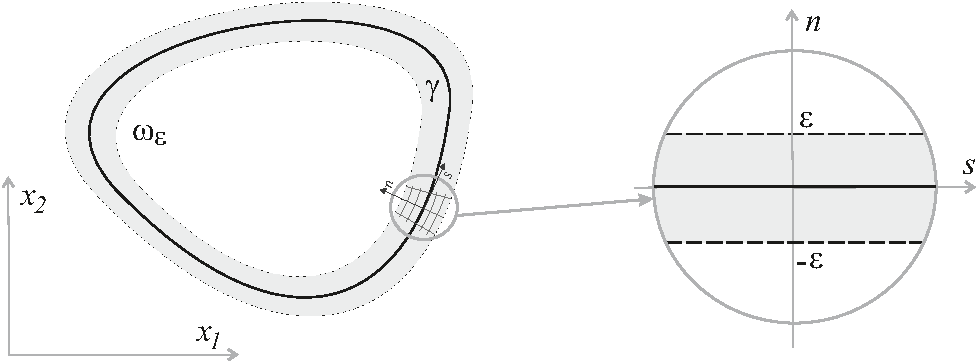
\includegraphics[scale=.6]{LocalCoords}
\caption{Curvilinear coordinates in the $\eps$-neighbourhood of $\gamma$.}
\label{FigLocalCoords}
\end{figure}


We suppose that the localized potentials have the following structure
\begin{equation}\label{Veps}
V_\eps(\alpha(s)+r\nu(s))=\eps^{-2}\,V\left(\eps^{-1}r\right)
+\eps^{-1}\,U\left(s,\eps^{-1}r\right),
\end{equation}
where $V$ and $U$ are measurable bounded functions such that
\begin{equation}\label{pdsU}
\supp V\subset (-1,1), \quad \supp U\subset Q_1 \mbox{ and }\partial_s U\in L_2(\Real^2).
\end{equation}
 The key assumption is that $V$ does not depend on  $s$.

The family of potentials $V_\eps$ generally diverges in the space of distributions $\mathcal{D}(\Real^2)$.
As we will show  in Propositin~\ref{PropVepsConverg},
the  potentials converge only if $V$ is a zero mean function. In this case,
$V_\eps\to a \partial_\nu\delta_\gamma+b\delta_\gamma$ as $\eps\to 0$ for some functions $a$ and $b$,
where $\delta_\gamma$ is the Dirac delta function supported on $\gamma$ and $\partial_\nu\delta_\gamma$ is the normal derivative of $\delta_\gamma$ at points of $\gamma$. More precisely,
\begin{equation*}
  \langle a\partial_\nu\delta_\gamma+b \delta_\gamma, \phi \rangle= -\int_\gamma  \npt(a\phi)\,d\gamma+\int_\gamma b \phi\,d\gamma
\end{equation*}
for all $\phi\in C^\infty_0(\Real^2)$.

The main task is to construct asymptotic approximations, as $\eps\to 0$, to eigenvalues  and eigenfunctions of $H_\eps$, i.e., asymptotics of eigenvalues $\lambda^\eps$ and eigenfunctions $u_\eps$ of spectral equation
\begin{equation}\label{SpectralEqn}
-\Delta u_\eps +(W+V_\eps) u_\eps= \lambda^\eps u_\eps\quad \hbox{in \ } \Real^2.
\end{equation}





We  introduce some notation. The plane is divided into two domains by close curve $\gamma$.  We suppose that $\Real^2\setminus\gamma=\Omega_{in}\cup\Omega_{out}$, where domain $\Omega_{out}$ is unbounded. Also, we say that $v$ belongs to space $\mathcal{V}\subset L_2(\Real^2)$ if $v|_{\Omega_-}\in W_2^2(\Omega_{in})$ and there exist a function $w$ belonging to $\dom H_0$ such that $v=w$ in $\Omega_{out}$. Of course, $v|_{\Omega_{out}}\in W_{2,loc}^2(\Omega_{out})$.
Let $\mathcal{V}_0$ be the subspaces of $L_2(\Omega_{out})$
obtained by the restriction of all elements of $\mathcal{V}$ to $\Omega_{out}$.   We introduce two operators
\begin{align*}
&\mathcal{D}_1= -\Delta+W, \qquad \dom \mathcal{D}_1=\{v\in \mathcal{V}_0\colon\; v=0 \;\,\mbox{on } \gamma\},\\
&\mathcal{D}_2= -\Delta+W, \qquad \dom \mathcal{D}_2=\{v\in W_2^2(\Omega_{in})\colon\; v=0 \;\,\mbox{on } \gamma\}.
\end{align*}


We also denote by $\gamma_t=\{x\in\Real^2\colon\; x=\alpha(s)+t\nu(s), \; s\in S\}$ the closed curve that is obtained from $\gamma$ by flowing for ``time'' $t$ along the normal vector field. Then the boundary of $\omega_\eps$ consists of two curves $\gamma_{-\eps}$ and $\gamma_{\eps}$. For each $u\in \mathcal{V}$ there exist two one-side traces on $\gamma$, namely
\begin{equation}\label{UpmNotation}
  u^-=\lim_{\eps\to 0}u|_{\gamma_{-\eps}}, \qquad
u^+=\lim_{\eps\to 0}u|_{\gamma_{\eps}}.
\end{equation}







We say that the Schr\"odinger operator~$-\frac{d^2}{d t^2}+V$ in $L_2(\Real)$ possesses a \emph{zero-energy resonance}  if there exists a non trivial solution~$h$ of the equation $-h'' +Vh= 0$ that is bounded on the whole line.  We call $h$ the \emph{half-bound state} of $V$. In this case, we will also simply say that potential $V$ has a half-bound state $h$. Such a solution~$h$ is  unique up to a scalar factor and has nonzero limits
\begin{equation*}
  h(-\infty)=\lim\limits_{t\to-\infty}h(t), \qquad
  h(+\infty)=\lim\limits_{t\to+\infty}h(t)
\end{equation*}
at both the infinities. We set
\begin{equation}\label{Theta}
  \theta=\frac{h(+\infty)}{h(-\infty)}.
\end{equation}



Our main result reads as follows.


\begin{thm}\label{MainThrm}
Let $W\in L^\infty_{loc}(\Real^2)$ and  $\dom H_0\subset W_2^1(\Real^2)$.
Assume  that potentials $V$ and $U$  are measurable bounded functions and assumption \eqref{pdsU} and \eqref{Vzeromean}  holds.
Then the family of operators
\begin{equation*}
 H_\eps=-\Delta +W+V_\eps,
\end{equation*}
where the perturbation $V_\eps$ is given by \eqref{Veps},
converges as $\eps\to 0$ in the strong resolvent sense.

If potential $V$ possesses a zero-energy resonance with a half-bound state $h$, then operators $H_\eps$ converge to  operator $\mathcal{H}$
defined by
$
\mathcal{H} v=-\Delta v+Wv
$
on functions $v\in \mathcal{V}$  obeying the interface conditions
\begin{equation}\label{ConnectedCond}
 u^+-\theta u^-=0,\quad  \theta\partial_\nu u^+-\partial_\nu u^-
=\left(\textstyle\frac{1}{2 }(\theta^2-1)\kappa+\mu\right) u^-
\end{equation}
on curve $\gamma$. Here  $\theta$ is given by  \eqref{Theta},  $\kappa$ is the signed curvature of $\gamma$, and
\begin{equation}\label{Mu}
  \mu=\frac{1}{h^2(-\infty)} \int_{-1}^1 U(\,\cdot\,,t)h^2(t)\, dt.
\end{equation}


If potential $V$ has no zero-energy resonance, then operators $H_\eps$ converge to the direct sum $\mathcal{D}_1\oplus\mathcal{D}_2$ of two unperturbed operators $-\Delta +W$ in $\Omega_{in}$ and $\Omega_{out}$ respectively with the Dirichlet boundary conditions on interface $\gamma$.
\end{thm}


\begin{rem}
  If potential $V$ is identically zero, then $V_\eps=\eps^{-1}\,U\left(s,\eps^{-1}n\right)$ and so obviously
$V_\eps\to \mu_0 \delta_\gamma$, as $\eps\to 0$, in the space of distributions. Here
\begin{equation}\label{Mu0}
  \mu_0(s)=\int_{-1}^1U(s,t)\, dt.
\end{equation}
Potential $V=0$ possesses a zero-energy resonance with constant functions as  half-bound states. Hence parameter $\theta$ equals  $1$ and interface conditions \eqref{ConnectedCond} become
$ u^+- u^-=0$,  $\partial_\nu u^+-\partial_\nu u^-
-\mu_0 u^-=0$. These conditions are exactly the same as that obtained in \cite{BehrndtExnerHolzmannLotoreichik2017}.
\end{rem}






%%%%%%%%%%%%%%%%%%%%%%%%%%%%%%%%%%%%%%%%%%%%%%%%%%%%%%%%%%%%%%%%%%%%%%%%%%
% Preliminaries
%%%%%%%%%%%%%%%%%%%%%%%%%%%%%%%%%%%%%%%%%%%%%%%%%%%%%%%%%%%%%%%%%%%%%%%%%%

\section{Preliminaries}

Returning now to curvilinear coordinates $(s,r)$ given by \eqref{LocalTr},
we see that the couple of vectors
$ \tau=(\dot{\alpha}_1, \dot{\alpha}_2)$, $\nu=(-\dot{\alpha}_2, \dot{\alpha}_1)$
gives a Frenet frame for $\gamma$.
The Jacobian of transformation $x=\alpha(s)+r\nu(s)$ has the form
\begin{multline*}
J(s,r)=
\begin{vmatrix}
  \dot{\alpha}_1(s)-r\ddot{\alpha}_2(s)& -\dot{\alpha}_2(s)\\
          \dot{\alpha}_2(s)+r\ddot{\alpha}_1(s)\phantom{0} & \dot{\alpha}_1(s)
\end{vmatrix}
\\
=\dot{\alpha}_1^2(s)+\dot{\alpha}_2^2(s)
-r\big(\dot{\alpha}_1(s)\ddot{\alpha}_2(s)-
  \dot{\alpha}_2(s)\ddot{\alpha}_1(s)\big)=1-r \kappa(s).
\end{multline*}
Here $\kappa=\det(\dot{\alpha},\ddot{\alpha})$ is the signed curvature of $\gamma$. Note that $\kappa$ is a continuous function
of the arc-length parameter $s$ and the sign of $\kappa(s)$ is defined uniquely up to the re-parametrization $s\mapsto-s$.
We see that $J$ is positive for sufficiently small $n$, because  curvature $\kappa$  is  bounded on $\gamma$.
Namely, the curvilinear coordinates $(s,r)$ can be defined correctly on all domains $\omega_\eps$ with $\eps\leq \eps_*$, where
$\eps_*=\min_{\gamma}|\kappa|^{-1}$.
However, the above we have accepted that $\eps_*=1$, since this
involves no loss of generality. We also have
\begin{equation}\label{IntegralCh}
  \int_{\omega_\eps} f(x_1,x_2)\,dx_1dx_2=\int_{Q_\eps} f(s,r)(1-r\kappa(s))\,ds\,dr
\end{equation}
for all integrable functions $f$.
The metric tensor $g=(g_{ij})$ of $\omega_\eps$ in the orthogonal coordinates $(s,r)$  has the form
  \begin{equation*}
    g=
    \begin{pmatrix}
      J^2\phantom{0} & 0 \\
          0\phantom{0} & 1
    \end{pmatrix}.
  \end{equation*}
In fact, we have
$g_{11}=|x_s|^2=|\dot{\alpha}+r \dot{\nu}|^2
=|(1-r\kappa) \dot{\alpha}|^2=J^2$,
by the Frenet-Serret formula $\dot{\nu}=-\kappa \dot{\alpha}$, and $g_{22}=|x_r|^2=|\nu|^2=1$.
In particular,  the gradient in the local coordinates becomes
\begin{equation*}
 \nabla \phi=\frac1{\sqrt{g_{11}}}\,\partial_s\phi\, \tau+\frac1{\sqrt{g_{22}}}\,\partial_r\phi\, \nu=\frac1J\,\partial_s\phi\, \tau+\partial_r\phi\, \nu
\end{equation*}
and  therefore we have
\begin{equation}\label{ScalarProdGrads}
  \nabla \phi\cdot \nabla \psi=J^{-2}\partial_s\phi\, \partial_s \psi+
\partial_r \phi\; \partial_r \psi.
\end{equation}
The Laplace-Beltrami operator in $\omega_\eps$ has also the explicit form
\begin{equation}\label{LaplacianInSN}
\Delta \phi=J^{-1}\left(\partial_s(J^{-1}\partial_s \phi)+ \partial_r(J\partial_r \phi)\right)
\end{equation}
as is easy to check.
%
%Notwithstanding the title of paper, all results presented in the article concern the potentials $V_\eps$ with arbitrary functions $V$ and $U$ of compact support, and $V_\eps$ generally diverge in the distributional sense. Therefore
%the $(a \partial_\nu\delta_\gamma+b\delta_\gamma)$-like potentials are only a partial case in our considerations. However,
%surprisingly enough, without reference to the convergence of $V_\eps$  the limit of $H_\eps$ exists in the strong resolvent sense. It is also worth noting that the convergence conditions for potentials $V_\eps$ and operators $H_\eps$ are quite different. In particular, the convergence of potentials does not depend on the existence of zero-energy resonances for $V$.


\begin{prop}\label{PropVepsConverg}
If $\int_\Real V\,dt=0$, then
\begin{equation*}
   V_\eps\to \beta\partial_\nu\delta_\gamma+\left(\beta\kappa+\mu_0\right) \delta_\gamma,\quad \mbox{as } \eps\to 0,
\end{equation*}
in the space of distributions $\mathcal{D}'(\Real^2)$, where
$\beta=-\int_\Real t V(t)\,dt$ and $\mu_0$ is given by \eqref{Mu0}.
\end{prop}
\begin{proof}
It is evident that potentials $\eps^{-1}\,U\left(s,\eps^{-1}r\right)$
converge to $\mu_0 \delta_\gamma$ in $\mathcal{D}(\Real^2)$.
We will prove that sequence $g_\eps=\eps^{-2}\,V\left(\eps^{-1}r\right)$ converges to
$\beta\left(\partial_\nu\delta_\gamma+\kappa\delta_\gamma\right)$ as $\eps\to 0$, provided $V$ is a zero-mean function.
In fact, for all $\phi\in C^\infty_0(\Real^2)$ we have
\begin{multline*}
\langle g_\eps, \phi \rangle=\int_{\omega_\eps}g_\eps(x)\phi(x)\,dx
=
\frac{1}{\eps^2}\int_{Q_\eps} V\left(\frac{r}{\eps}\right)\phi(s,r)(1-r\kappa(s))\,ds\,dr
\\
 =
\frac{1}{\eps}\int_{Q_1} V(t)\phi(s,\eps t)(1-\eps t\kappa(s))\,ds\,dt
\\
=\frac{1}{\eps}\int_{-1}^1 V(t)\,dt \int_S\phi(s,0)\,ds
\\
+
\int_{-1}^1 t V(t)\,dt \int_S\big(\partial_n\phi(s,0)-\kappa(s)\phi(s,0)\big)\,ds+O(\eps),
\end{multline*}
as $\eps\to 0$.
The sequence $\langle g_\eps, \phi \rangle$ has a finite limit for all $\phi\in C^\infty_0(\Real^2)$ if and only if $\int_\Real V\,dt=0$.
In this case, we have
\begin{equation*}
\langle g_\eps, \phi \rangle\to \beta\int_\gamma\left(\partial_\nu\delta_\gamma+\kappa \delta_\gamma\right)\phi\,d\gamma,
\end{equation*}
which completes the proof.
\end{proof}

Interface conditions \eqref{ConnectedCond} contain the parameters which depend on the particular parametrization chosen for curve $\gamma$. More precisely, parameters $\theta$, $\kappa$ and $\mu$ change along with the change of the Frenet frame.

\begin{prop}\label{PropInvarianceOfCnds}
  Operator $\mathcal{H}$ in Theorem~\ref{MainThrm} does not depend upon the choice of the Frenet frame for curve $\gamma$.
\end{prop}
\begin{proof}
Every smooth curve in the plane admits two possible orientations of arc-length parameter and consequently two possible  Frenet frames. Let us change the Frenet frame $\{\tau, \nu\}$, previously introduced in Sec.~\ref{Sec:Statment}, to the frame $\{-\tau, -\nu\}$ and prove that
interface conditions \eqref{ConnectedCond} will remain the same. This change leads to the following transformations:
\begin{gather*}
h(\pm\infty)\mapsto h(\mp\infty), \quad u_\pm\mapsto u_\mp, \quad \partial_\nu u_\pm \mapsto -\partial_\nu u_\mp,\\
\theta\mapsto \theta^{-1}, \quad \kappa\mapsto -\kappa,\quad \mu\mapsto \theta^{-2}\mu.
\end{gather*}
The first condition $u^+-\theta u^-=0$ in \eqref{ConnectedCond} transforms into $u^--\theta^{-1} u^+=0$ and therefore remains unchanged. As for the second condition, we have
\begin{equation*}
 	-\theta^{-1}\partial_\nu u^-+\partial_\nu u^+
	-\left(-\textstyle\frac{1}{2}(\theta^{-2}-1)\kappa
	+\theta^{-2}\mu\right) u^+=0.
\end{equation*}
Multiplying the equality by $\theta$  yields
\begin{equation*}
	\theta\partial_\nu u^+-\partial_\nu u^-
	-\left(\textstyle\frac{1}{2 }(\theta^{2}-1)\kappa+\mu\right) 	\theta^{-1} u^+=0,
\end{equation*}
since $-\theta(\theta^{-2}-1)=\theta^{-1}(\theta^{2}-1)$. It remains to insert $u^-$ in place of $\theta^{-1} u^+$, in view of the first interface condition.
\end{proof}

In the sequel, the normal vector field $\nu$ will be outward to domain $\Omega_{in}$, that is to say, the local coordinate $n$ will increase in the direction from $\Omega_{in}$ to $\Omega_{out}$.
At the end of the section,  we record some technical assertion, which  will be often used below.
Throughout the paper, $W_2^l(\Omega)$ stands for the Sobolev space of functions defined on a set $\Omega$.



\begin{prop}\label{PropTrace}
Suppose that $v\in W_2^{1}(\Omega_{out})$  and $w\in W_2^{1}(\Omega_{in})$. Then
\begin{align}\label{EstVeps-V0}
&\|v(\,\cdot\,,\eps)-v(\,\cdot\,,0)\|_{L_2(\gamma)}\leq
c_1\eps^{1/2}\|v\|_{W_2^1(\Omega_{out})}, \\\label{EstWeps-W0} &\|w(\,\cdot\,,-\eps)-w(\,\cdot\,,0)\|_{L_2(\gamma)}\leq
c_2\eps^{1/2}\|w\|_{W_2^1(\Omega_{in})},
\end{align}
where the constants $c_k$ do not depend on $\eps$.
\end{prop}
\begin{proof}
First we assume that $v$ is a smooth function in $\Omega_{out}$. Then
\begin{equation*}
 v(s,\eps)-v(s,0)=\int_0^\eps \partial_t v(s,t)\,dt,
\end{equation*}
and for all $\psi\in L_2(\gamma)$ we have
\begin{equation*}
\int_S(v(s,\eps)-v(s,0))\psi(s)\,ds=\int_S\int_0^\eps\partial_t v(s,t)\psi(s)\,dt\,ds.
\end{equation*}
Therefore
\begin{multline*}
\left|\int_S\big(v(s,\eps)-v(s,0)\big)\psi(s)\,ds\right|\leq
\int_S\int_0^\eps|\partial_t v(s,t)|\,|\psi(s)|\,dt\,ds
\\
\leq \left(\int_0^\eps \int_S|\psi(s)|^2\,ds\,dt\right)^{1/2}
\left(\int_S\int_0^\eps |\partial_t v|^2\,dt\,ds\right)^{1/2}
\\
\leq c\eps^{1/2}\|\psi\|_{L_2(\gamma)}
\left(\int_{\Omega_{out}}|\nabla v|^2\,dx\right)^{1/2}\leq c_1\eps^{1/2}\|v\|_{W_2^1(\Omega_{out})}\|\psi\|_{L_2(\gamma)}.
\end{multline*}
Hence \eqref{EstVeps-V0} holds for all smooth functions $v$ and then by continuity for all $v\in W_2^{1}(\Omega_{out})$.
Similar arguments apply to the proof of \eqref{EstWeps-W0}.
\end{proof}


%%%%%%%%%%%%%%%%%%%%%%%%%%%%%%%%%%%%%%%%%%%%%%%%%%%%%%%%%%%%%%%%%%%%%%%%%%
% Calculation of Limit Operator
%%%%%%%%%%%%%%%%%%%%%%%%%%%%%%%%%%%%%%%%%%%%%%%%%%%%%%%%%%%%%%%%%%%%%%%%%%

\section{Formal Asymptotics}
\subsection{Leading Terms}
\label{Sec:LimitOperator}

In this section we will show how interface conditions \eqref{ConnectedCond} can be found by direct calculations, constructing the formal asymptotics of  eigenvalues and eigenfunctions.
We  look for asymptotics of $\lambda_\eps$ and $u_\eps$ in the form
\begin{equation}\label{AsymptoticsUe}
\lambda^\eps\approx \lambda+\eps \lambda_1, \qquad u_\eps(x)\approx
\begin{cases}
  u(x)+\eps u_1(x)& \hbox{in \ }\Real^2\setminus \omega_\eps, \\
    v_0\left(s,\nep\right)+\eps v_1\left(s,\nep\right)+\eps^2 v_2\left(s,\nep\right)
&\hbox{in \ } \omega_\eps.
\end{cases}
\end{equation}
Recall that the boundary of $\omega_\eps$ consists of  two curves
$\gamma_{-\eps}$ and $\gamma_{\eps}$.
To match two different approximations, we hereafter assume that
\begin{equation}\label{MatchingCnds}
  [u_\eps]_{\gamma_{\pm\eps}}=0, \quad [\partial_\nu u_\eps]_{\gamma_{\pm\eps}}=0,
\end{equation}
where $[\,\cdot\,]_{\gamma_{\pm\eps}}$ is a jump  across $\gamma_{\pm\eps}$.
Since function $u_\eps$ solves \eqref{SpectralEqn} and domain $\omega_\eps$ shrinks to $\gamma$, the leading term $u$ must be a solution of the equation
\begin{equation*}
-\Delta u+Wu= \lambda u \quad \hbox{in \ } \Real^2\setminus \gamma,
\end{equation*}
subject to appropriate interface conditions on $\gamma$.
To find these conditions, we consider equation \eqref{SpectralEqn} in the curvilinear coordinates $(s,n)$, where $n=r/\eps$. Then in vicinity of $\gamma$ the Laplacian can be written as
\begin{equation}
  \Delta =\frac1{1-\eps n\kappa}\left( \eps^{-2}\partial_n
  (1-\eps n\kappa)\partial_n +\partial_s
  \Big(\frac1{1-\eps n\kappa}\,\partial_s\Big)\right),
\end{equation}
by \eqref{LaplacianInSN}.
From this we readily deduce the asymptotic representation
\begin{equation*}
\Delta= \eps^{-2}\partial^2_n-\eps^{-1}\kappa\partial_n
-n\kappa^2\partial_n+\partial^2_s+\eps P_\eps,
\end{equation*}
where $P_\eps$ is a partial differential operator on the second order with respect to $s$ and the first one with respect to $n$ whose coefficients  are uniformly bounded on $\eps$.
Substituting \eqref{AsymptoticsUe} into \eqref{SpectralEqn} for $x\in \omega_\eps$ in particular yields
\begin{equation}\label{EqnsV0V1}
-\pte^2 v_0+V(n)v_0=0,
\qquad
-\pte^2 v_1+V(n)v_1=-\kappa(s)\pte v_0-U(s,n)v_0
\end{equation}
in cylinder $Q_1=S\times(-1,1)$.
From \eqref{MatchingCnds} we see that necessarily
\begin{gather}\label{FittingCndsUV0}
 u^-(s)=v_0(s,-1),\qquad u^+(s)=v_0(s,1),
 \\\label{FittingCndspV0}
 \partial_n v_0(s,- 1)=0, \qquad \partial_n v_0(s, 1)=0, \\\label{FittingCndspV1}
 \partial_n v_1(s, -1)=\partial_\nu u^-(s), \qquad
 \partial_n v_1(s, 1)=\partial_\nu u^+(s),
\end{gather}
where $u^\pm$ are defined by \eqref{UpmNotation}.
Combining \eqref{FittingCndspV0}--\eqref{FittingCndspV1}, we conclude that $v_0$ and $v_1$ solve boundary value problems
\begin{align}\label{problemV0}
&\begin{cases}
  -\pte^2 v_0+V(n)v_0=0 \quad \hbox{in \ } Q_1, \\
    \phantom{-}\partial_n v_0(s,- 1)=0, \quad \partial_n v_0(s, 1)=0, \quad s\in S;
\end{cases}
\\\label{problemV1}
&\begin{cases}
  -\pte^2 v_1+V(n)v_1=-\kappa(s)\pte v_0-U(s,n)v_0\quad \hbox{in \ } Q_1, \\
    \phantom{-}\partial_n v_1(s, -1)=\partial_\nu u^-(s), \quad
\partial_n v_1(s, 1)=\partial_\nu u^+(s), \quad s\in S
\end{cases}
\end{align}
respectively.
We have two boundary value problems for the ``non-ellip\-tic'' partial differential operator in $Q_1$. Of course,  the problems can also be  regarded as  boundary value problems for ordinary differential equations on $(-1,1)$, which depend on parameter $s\in S$.



%
%In fact, let $\ell$ be the length of $S$ and then the length of $\gamma$. Then both problems \eqref{problemV0} and  \eqref{problemV1} can write out as  boundary value problem in  rectangle $\Pi=(0,\ell)\times(-1,1)$
%\begin{equation*}
%  \begin{cases}
%    -\pte^2 v+V(t)v=g(s,n), \qquad (s,n)\in \Pi, \\
%    \phantom{-}\partial_t v(s,- 1)=a_-(s), \quad \partial_t v(s, 1)=a_+(s), \quad s\in S,\\
%\phantom{-}v(0,t)=v(\ell,t), \quad \partial_s v(0,t)=\partial_s v(\ell,t), \quad t\in (-1,1)
%  \end{cases}
%\end{equation*}
%with the Neumann boundary conditions with respect to $t$ and the periodicity conditions with respect to $s$.
%In any case, the lack of ellipticity  leads to a loss of smoothness of solutions with respect to $s$, and this will have an considerable influence on the proof of Theorem~\ref{MainThrm}.
%



















\textit{Case of zero-energy resonance.}
Assume that operator $-\frac{d^2}{dt^2}+V$ has a zero energy resonance with half-bound state $h$. Since the support of $V$ lies in  interval $(-1,1)$, the half-bound state $h$ is  constant  outside this interval as a bounded solution of equation $h''=0$.
Therefore the restriction of $h$ to $(-1,1)$ is a nonzero solution of the Neumann boundary value problem
\begin{equation}\label{NeumanProblem}
     -h''+V(n)h= 0,\quad n\in(-1,1),\qquad   h'(-1)=0, \quad h'(1)=0.
\end{equation}
Hereafter, we fix $h$ by additional condition $h(-1)=1$. In view of
\eqref{Theta}, we have $h(1)=\theta$, since $h(\pm\infty)=h(\pm 1)$.




In this case, \eqref{problemV0}  admits a infinite-dimensional space of solutions
\begin{equation*}
\mathcal{N}=\big\{a(s)h(n)\colon \;a\in L^2(S)\big\}.
\end{equation*}
Therefore $v_0(s,n)=a_0(s)h(n)$ for some function $a_0$. From \eqref{FittingCndsUV0} we deduce that $u^-=a_0$ and $u^+=\theta a_0$ and hence that
\begin{equation}\label{RCond0}
     u^+=\theta u^-\quad\text {on }\gamma.
\end{equation}
In addition, we must set $v_0(s,n)=u^-(s)h(n)$.


Problem \eqref{problemV1} is in general unsolvable, since $\mathcal{N}\neq\{0\}$.  To find solvabi\-li\-ty conditions, we rewrite  equation in \eqref{problemV1} as
\begin{equation}\label{eqnV1Expand}
  -\pte^2 v_1+V(n)v_1=-\big(\kappa(s)h'(n)+U(s,n)h(n)\big)u^-(s),
\end{equation}
multiply  by an arbitrary element of  $\mathcal{N}$  and then integrate over $Q_1$
\begin{multline}\label{IntV1H}
\int_{Q_1}\left(-\pte^2 v_1+V(n)v_1\right)a(s)h(n)\,dn\,ds
\\
=
-\int_{Q_1}(\kappa(s)h'(n)+U(s,n)h(n))u^-(s)a(s)h(n)\, dn\,ds.
\end{multline}
Since $h$ is a solution of \eqref{NeumanProblem}, integrating by parts twice on the left-hand side yields
\begin{multline*}
\int_{S} \int_{-1}^1\left(-\pte^2 v_1+Vv_1\right)a h\,dn \,ds
=-\int_{S}( \partial_n v_1 h-v_1 h')\big|_{n=-1}^{n=1}a\,ds\\-
\int_{S} \int_{-1}^1 a v_1\left(-h''+Vh\right)\,dn\,ds
=-\int_{S}\big(\theta\partial_\nu u^+-\partial_\nu u^-\big) a\,ds,
\end{multline*}
in view of the boundary conditions for $v_1$.
Recall that $h(-1)=1$ and $h(1)=\theta$.
Since $hh'=\frac12 (h^2)'$, we also have $\int_{-1}^1hh'\,d t=\textstyle\frac{1}{2 }(\theta^2-1)$.
Therefore \eqref{IntV1H} becomes
\begin{equation*}
\int_{S}\left(\theta\partial_\nu u^+-\partial_\nu u^-\right)a\,ds
=\int_{S}\big(\textstyle\frac{1}{2}(\theta^2-1)\kappa+\mu \big)u^-a\,ds
\end{equation*}
for all  $a\in L^2(S)$, where $\mu(s)=\int_{-1}^1 U(s,n)h^2(n)\, dn$.
Therefore
\begin{equation*}
  \theta\partial_\nu u^+-\partial_\nu u^-
=\big(\textstyle\frac{1}{2}(\theta^2-1)\kappa+\mu \big) u^-\quad\text {on }\gamma,
\end{equation*}
which is necessary for the solvability of \eqref{problemV1}.
In view of the Fredholm alternative, this condition is also a sufficient one. At the same time, it is a jump condition at the interface $\gamma$ for the normal derivative of $u$.

Therefore the leading terms $\lambda$ and $u$ of asymptotics \eqref{AsymptoticsUe} solve the problem
\begin{gather}\label{LimitProblemEq}
-\Delta u+Wu=\lambda u \qquad \hbox{in  } \Real^2\setminus \gamma,
\\ \label{RConds}
 \phantom{-}u^+-\theta u^-=0,  \quad
\theta\partial_\nu u^+-\partial_\nu u^-
=\big(\textstyle\frac{1}{2}(\theta^2-1)\kappa+\mu \big) u^- \quad \hbox{on } \gamma.
\end{gather}
Assume that $\lambda$ is an eigenvalue of operator $\cH$ associated with eigenfunction $u$. Now we can calculated the trace $u^-$ on $\gamma$ and  finally determine $v_0(s,n)=u^-(s)h(n)$.

\textit{Non-resonant case.}
Now suppose that problem \eqref{NeumanProblem} admits the trivial solution only, i.e.,  $\mathcal{N}=\{0\}$.  Then $v_0=0$ and therefore $u^-=0$ and $u^+=0$ on $\gamma$, by \eqref{FittingCndsUV0}. We thus get
\begin{equation*}
-\Delta u+Wu=\lambda u\quad \hbox{in \ } \Real^2\setminus \gamma,\qquad
 u|_{\gamma}=0.
\end{equation*}
Let us suppose that $\lambda$ is an eigenvalue of the direct sum
$\mathcal{D}_1\oplus\mathcal{D}_2$ of two Dirichlet type operators and $u$ is a corresponding eigenfunction.
In this case, problem \eqref{problemV1} has the form
\begin{equation}\label{problemV1Non}
\begin{cases}
    -\pte^2 v_1+V(n)v_1=0\quad \hbox{in \ } Q_1, \\
    \phantom{-}\partial_n v_1(s, -1)=\partial_\nu u^-, \qquad
\partial_n v_1(s, 1)=\partial_\nu u^+,
\end{cases}
\end{equation}
and admits a unique solution.


\subsection{Correction terms}
Upon our substituting \eqref{AsymptoticsUe} into  equation \eqref{SpectralEqn} and conditions \eqref{MatchingCnds},  we in particular discover that  correction term $u_1$ solves the equation
\begin{equation}\label{EqnU1}
 -\Delta u_1+Wu_1=\lambda u_1+\lambda_1 u\quad \hbox{in \ } \Real^2\setminus \gamma
\end{equation}
and $v_2$ is a solution of the problem
\begin{align}
&\begin{aligned}\label{problemV2eqn}
  -\pte^2 v_2+V(n)v_2=-(\kappa(s)&\pte +U(s,n)) v_1\\
  &+(\partial^2_s-n\kappa^2\partial_n-W(s,0)+\lambda)v_0
  \quad \hbox{in \ } Q_1,
\end{aligned}
\\\label{problemV2conditions}
 & \phantom{-} \partial_n v_2(\,\cdot\,, -1)=\partial_\nu u_1^--\partial_\nu^2 u^-,
 \quad
 \partial_n v_2(\,\cdot\,, 1)=\partial_\nu u_1^++\partial_\nu^2 u^+, \quad s\in S.
\end{align}
In addition,
\begin{equation}\label{CondsV1U1}
v_1(\,\cdot\,,-1)=u_1^--\partial_\nu u^-, \qquad
v_1(\,\cdot\,,1)=u_1^++\partial_\nu u^+.
\end{equation}


If operator $-\frac{d^2}{dt^2}+V$ has a zero energy resonance, then $u$ is an eigenfunction of \eqref{LimitProblemEq}, \eqref{RConds}.
 Since the second condition in \eqref{RConds} holds,
problem \eqref{problemV1} is solvable and possesses a li\-near manifold of solutions
\begin{equation}\label{RepresV1}
  v_1(s,n)=a_1(s) h(n)+ w(s,n), \qquad a_1\in L_2(S),
\end{equation}
where $w$ is a partial solution of \eqref{problemV1} such that $w(s,-1)=0$ for all $s\in S$.
We may therefore substitute \eqref{RepresV1} into \eqref{CondsV1U1} and obtain
\begin{equation*}
  a_1=u_1^--\partial_\nu u^-, \quad
  \theta a_1+ w(\,\cdot\,,1)=u_1^++\partial_\nu u^+,
\end{equation*}
from which the coupling condition
\begin{equation}\label{RCondU10}
  u_1^+-\theta u_1^-=w(\,\cdot\,,1)-\partial_\nu u^+-\theta\partial_\nu u^-\quad\text {on }\gamma
\end{equation}
follows. Also, we have $v_1(s,n)=(u_1^-(s)-\partial_\nu u^-(s)) h(n)+ w(s,n)$.


By reasoning similar to that for  \eqref{problemV1}, we can write the solvability condition for problem \eqref{problemV2eqn}, \eqref{problemV2conditions} as
\begin{equation}\label{RCondU11}
    \theta\partial_\nu u_1^+-\partial_\nu u_1^-
-\big(\textstyle\frac{1}{2}(\theta^2-1)\kappa+\mu \big) u_1^-=
 -\theta\partial^2_\nu u^+-\partial^2_\nu u^-+\int_{-1}^1f(s,n)h(n)\,dn,
\end{equation}
where $f=(\kappa\pte +U)( h\partial_\nu u_1^--w)+(\partial^2_s- n\kappa^2\partial_n-W(\,\cdot\,,0)+\lambda)v_0$.
Then \eqref{EqnU1}, \eqref{RCondU10} and\eqref{RCondU11} taken together yield
\begin{gather}\label{ProblemU1eqn}
  -\Delta u_1+Wu_1=\lambda u_1+\lambda_1 u\quad \hbox{in \ } \Real^2\setminus \gamma, \\\label{ProblemU1conds}
  u_1^+-\theta u_1^-=g_0, \quad
  \theta\partial_\nu u_1^+-\partial_\nu u_1^-
  -\big(\textstyle\frac{1}{2}(\theta^2-1)\kappa+\mu \big) u_1^-=g_1 \quad\text {on }\gamma,
\end{gather}
where $g_0$ and $g_1$ stand for the right hand sides of \eqref{RCondU10} and \eqref{RCondU11} respectively.

Since $\lambda$ is an eigenvalue of $\cH$, the last problem is generally unsolvable. But there exists a unique value of $\lambda_1$ for which \eqref{ProblemU1eqn}, \eqref{ProblemU1conds} admits a solution. Let us
multiply equation \eqref{ProblemU1eqn} by eigenfunction $u$, and integrate over $\Real^2$, to find
\begin{equation}\label{Lambda1}
  \lambda_1=\|u\|_{L_2(\Real^2)}^{-2}\int_{\gamma}\big(g_1u^- -g_0 \partial_\nu u^+ \big) \,d\gamma,
\end{equation}
where we have integrated by parts in the term containing $\Delta u_1$:
\begin{multline*}
  -\int_{\Real^2}\Delta u_1 u\,dx=-\int_{\Omega_{out}}\Delta u_1 u\,dx-\int_{\Omega_{in}}\Delta u_1 u\,dx \\
  =\int_{\gamma}\big(\partial_\nu u_1^+u^+-\partial_\nu u_1^-u^--u_1^+\partial_\nu u^++u_1^-\partial_\nu u^-\big) \,d\gamma-\int_{\Real^2} u_1\Delta u\,dx.
\end{multline*}
Utilizing the coupling conditions for $u$ and $u_1$ on interface $\gamma$, we have obtained
\begin{multline*}
  -\int_{\Real^2}\Delta u_1 u\,dx+\int_{\Real^2} u_1\Delta u\,dx
  \\
  = \int_{\gamma}\big((\theta\partial_\nu u_1^+-\partial_\nu u_1^-)u^- -
  (\theta\partial_\nu u^+-\partial_\nu u^-)u_1^--g_0 \partial_\nu u^+ \big) \,d\gamma
  \\
   = \int_{\gamma}\big((Ru_1^-+g_1)u^- -
  Ru^-u_1^--g_0 \partial_\nu u^+ \big) \,d\gamma=\int_{\gamma}\big(g_1u^- -g_0 \partial_\nu u^+ \big) \,d\gamma,
\end{multline*}
where $R=\frac{1}{2}(\theta^2-1)\kappa+\mu$.






\subsection{Adjustment of asymptotics}

\begin{prop}[Smoothness of asymptotics]
  Let
\end{prop}
\begin{proof}
We set
\begin{equation}\label{RepresentV1}
  v_1(s,n)=\partial_\nu u^-(s)h_1(n)-u^-(s)h_2(s,n),
\end{equation}
where $h_1$ and $h_2$ solve the Cauchy problems
\begin{align}\nonumber
&-h_1''+V(n)h_1=0,\quad t\in (-1,1),\quad  h_1(-1)=0, \; h_1'(-1)=1,\\
&\begin{cases}
  -h_2''+V(n)h_2=\kappa(s)h'(n)+U(s,n)h(n),\quad n\in (-1,1),\\\label{problH2}
\phantom{-}h_2(s,-1)=0, \quad \partial_n h_2(s,-1)=0,\quad s\in S
\end{cases}
\end{align}
respectively.
We see at once that  $v_1$ of the form \eqref{RepresentV1} solves equation \eqref{eqnV1Expand} and satisfies boundary conditions $v_1(s,-1)=0$ and $\partial_t v_1(s, -1)=\partial_\nu u^-(s)$. Now we show that  condition $\partial_t v_1(s, 1)=\partial_\nu u^+(s)$ also holds.
Recall that half-bound state $h$ was fixed by  $h(-1)=1$. Then
the Lagrange identity $(h_1h'-h_1'h)|_{-1}^1=0$ implies  $h_1'(1)=\theta^{-1}$.
Next, multiplying the equation in \eqref{problH2} by $h$ and  integrating by parts twice yield
\begin{equation*}
 (h'h_2-h\,\partial_th_2)\big|_{-1}^1=\kappa(s)\int_{-1}^1hh'\,dn
  +\int_{-1}^1U(s,n)h^2(n)\, dn.
\end{equation*}
Hence we have $\theta \,\partial_th_2(s,1)=-\frac{1}{2}(\theta^2-1)\kappa(s)-\mu(s)$, and then
derive
\begin{multline*}
\partial_t v_1(s,1)=\partial_\nu u^-(s)\,h_1'(1)- u^-(s)\,\partial_th_2(s,1)\\
=\theta^{-1} \Big(\partial_\nu u^-(s)+\big(\textstyle\frac{1}{2 }(\theta^2-1)\kappa(s)+\mu(s)\big)u^-(s)\Big)=\partial_\nu u^+(s)
\end{multline*}
in view of interface conditions \eqref{RConds}.
\end{proof}





%%%%%%%%%%%%%%%%%%%%%%%%%%%%%%%%%%%%%%%%%%%%%%%%%%%%%%%%%%%%%%%%%%%%%%%%%%
% Proof of Theorem
%%%%%%%%%%%%%%%%%%%%%%%%%%%%%%%%%%%%%%%%%%%%%%%%%%%%%%%%%%%%%%%%%%%%%%%%%%

\section{Proof of Theorem \ref{MainThrm}}
\label{Sec:Proof}

We will provide a proof for the most interesting case when potential $V$ has a zero-energy resonance. The non-resonant case, which
is much easier, follows similarly. We must prove that
\begin{equation}\label{RHeToRH}
 (H_\eps-\zeta)^{-1}f\to (\mathcal{H}-\zeta)^{-1}f,\quad \mbox{as } \eps\to 0,
\end{equation}
for all $f\in L_2(\Real^2)$ and some $\zeta\in \Cmpl\setminus\Real$.
But the resolvents of $H_\eps$ are uniformly bounded on $\eps$, namely,
\begin{equation*}
     \|(H_\eps-\zeta)^{-1}\|\leq |\Im \zeta|^{-1}.
\end{equation*}
It will thus be sufficient to prove that  \eqref{RHeToRH} holds for
$f\in \cF$, where $\cF$ is some dense subset of $L_2(\Real^2)$. We suppose that $\cF=C^\infty_0(\Real^2\setminus\gamma)$.
%In fact,
%if $f\in L_2(\Real^2)$, $\{f_n\}_{n=1}^\infty\subset \cF$ and $f_n\to f$ in $L_2(\Real^2)$, then
%\begin{eqnarray}\nonumber
%\|R_\eps(\zeta)f&&\kern-4pt-\kern2ptR(\zeta)f\|_{L_2(\Real^2)}
%\leq
%\|R_\eps(\zeta)(f_n-f)\|_{L_2(\Real^2)}\\\nonumber
%&&+
%\|R(\zeta)(f_n-f)\|_{L_2(\Real^2)}
%+
%\|R_\eps(\zeta)f_n-R(\zeta)f_n\|_{L_2(\Real^2)}
%\\\nonumber
%&&\leq
%(\|R_\eps(\zeta)\|+\|R(\zeta)\|)\,\|f_n-f\|_{L_2(\Real^2)}
%+\|R_\eps(\zeta)f_n-R(\zeta)f_n\|_{L_2(\Real^2)},
%\end{eqnarray}
%and so the right-hand side tends to zero as $\eps\to 0$ and $n\to +\infty$. We write $R_\eps(\zeta)$ and  $R(\zeta)$ instead of $(H_\eps-\zeta)^{-1}$ and $(\mathcal{H}-\zeta)^{-1}$ respectively.

Hereafter, letters $c_j$ denote various posi\-ti\-ve numbers independent of~$\eps$, whose values might be different in different proofs.



\subsection{Approximation in $W_2^1(\Real^2)$}

Given $f\in \cF$ and $\zeta\in \Cmpl$, $\Im \zeta \neq 0$, we must compare $u_\eps=(H_\eps-\zeta)^{-1}f$ and $u=(\mathcal{H}-\zeta)^{-1}f$ in $L_2(\Real)$, and show that the difference $u_\eps-u$ is infinitely small in $L_2(\Real)$-norm, as $\eps\to 0$.
The basic idea of the proof is to construct a suitable approximation to $u_\eps$ in  $W_2^1(\Real^2)$.
The formal asymptotics \eqref{AsymptoticsWe} constructed above  will be used as a starting point in the construction of this approximation.
We recall that the Sobolev space $W_2^1(\Real^2)$ contains the domains
of $H_0$ and $H_\eps$.


We note that $v_0\in W_2^1(Q_1)$. This inclusion follows from the explicit form $v_0(s,t)=u^-(s)h(t)$, where  $u^-$ belongs to
$W_2^{3/2}(S)$ (as a trace of $u\in W_2^2(\Omega_{in})$  on curve  $\gamma$) and $h\in W_2^2(-1,1)\subset C^1(-1,1)$.
In view of representation formula \eqref{RepresentV1}, function $v_1$ does not belongs to $W_2^1(Q_1)$, since $\partial_\nu u^-\in W_2^{1/2}(S)$ in general.  However the term $u^- h_2$ in \eqref{RepresentV1} is an element of $W_2^1(Q_1)$, because $h_2=h_2(s,t)$ possesses the additional smoothness with respect to $s$ owing to the making more smoothness assumptions upon the curve $\gamma$ and potential $U$. Recall that $\kappa\in C^1(S)$ and $\partial_s U\in L_2(\Real^2)$.

We now regularize the trace $\partial_\nu u^-$.  Let $\{\beta_\eps^-\}_{\eps>0}$ be a sequence in $W_2^{1}(\gamma)$ such that $\beta_\eps^-\to  \partial_\nu u^-$ in  $W_2^{-1/2}(\gamma)$.
The sequence can be chosen in such a way that
\begin{equation}\label{EstBetaEps}
  \|\beta_\eps^--\partial_\nu u^-\|_{W_2^{-1/2}(\gamma)}\leq c_1 \eps^{1/2}\qquad   \|\beta_\eps^-\|_{W_2^1(\gamma)}\leq c_2 \eps^{-1/2},
\end{equation}
since $|\langle\beta_\eps^--\partial_\nu u^-,\,\beta_\eps^-\rangle|\leq
\|\beta_\eps^--\partial_\nu u^-\|_{W_2^{-1/2}(\gamma)}\|\beta_\eps^-\|_{W_2^{1}(\gamma)}
$
Then the function
\begin{equation}\label{representV1Eps}
    v_1^\eps(s,t)= \beta_\eps^-(s)h_1(t)-u^-(s)h_2(s,t)
\end{equation}
belongs to $W_2^1(Q_1)$ and solves the problem
\begin{equation}\label{ProblemV1eps}
\begin{cases}
   -\pte^2 v_1^\eps+V(t)v_1^\eps=-\kappa(s)u^-(s)h'(t)-U(s,t)h(t)\quad \hbox{in \ } Q_1, \\
    \phantom{-}\partial_t v_1^\eps(s, -1)=\beta_\eps^-(s), \quad
\partial_t v_1^\eps(s, 1)=\beta_\eps^+(s),\quad s\in S,
\end{cases}
\end{equation}
where $ \beta_\eps^+=\theta^{-1}
\left(\textstyle\frac{1}{2 }(\theta^2-1)\kappa u^--\beta_\eps^-\right)$.
Thus
\begin{equation}\label{BetaEpsPlus}
  \|\beta_\eps^+-\partial_\nu u^+\|_{W_2^{-1/2}(\gamma)}\leq c_1 \eps^{1/2},
\end{equation}
as $\eps\to 0$, by solvability condition \eqref{RCond1}. We also have the bounds
\begin{equation}\label{DerivOfV1Bounds}
  \|v_1^\eps\|_{L_2(Q_1)}+ \|\partial_t v_1^\eps\|_{L_2(Q_1)}\leq C_1,
   \qquad\|\partial_s v_1^\eps\|_{L_2(Q_1)}\leq C_2\eps^{-1/2}.
\end{equation}




















%
%\begin{lemma}\label{LemmaGradVk}
% The estimates
%\begin{equation}\label{EstV0inOmegaSmall}
%   \int_{\omega_\eps}|\nabla v_0(x_\eps)|^2\,dx
%   \leq C_0 \eps^{-1},\qquad
%   \int_{\omega_\eps}|\nabla v_1^\eps(x_\eps)|^2\,dx
%   \leq C_1 \eps^{-1-2\eta }
%\end{equation}
%hold, where $v_0(x_\eps)$ and $v_k^\eps(x_\eps)$ stand for $v_0(s,\nep)$ and $v_1^\eps(s,\nep)$ respectively.
%\end{lemma}
%\begin{proof}
% First, we note $dx_1dx_2=J(s,n)\,ds\,dn=\eps J_\eps(s,t)\,ds\,dt$,
%where $t=n/\eps$ and $J_\eps(s,t)=J(s,\eps t)=1-\eps t\kappa(s)$. In addition, for $v\in W_2^1(Q_1)$ we have
%\begin{equation}\label{LocalGrad}
% |\nabla v(x_\eps)|^2=\eps^{-2}|\partial_t v(s,t)|^2+J^{-2}_\eps(s,t)\,|\partial_s v(s,t)|^2,
%\end{equation}
%in view of \eqref{ScalarProdGrads}. Therefore
%\begin{eqnarray}\nonumber
%  \int_{\omega_\eps}|\nabla v(x_\eps)|^2\,dx
%  &&=\eps \int_{Q_1}\left(\eps^{-2}|\partial_t v|^2+J^{-2}_\eps\,|\partial_s v|^2
%\right)J_\eps\,ds\,dt\\\nonumber
% &&\leq c_1\eps^{-1} \int_{Q_1}\left(|\partial_t v|^2+\eps|\partial_s v|^2
%\right)\,ds\,dt \leq  c_2 \eps^{-1}\|v\|^2_{W_2^1(Q_1)},
%\end{eqnarray}
%since  $1/2\leq J_\eps(s,t) \leq 2$ for $\eps$ small enough.
%It remains to observe that $v_0$ belongs to $W_2^1(Q_1)$ and
%apply \eqref{EstBetaEps} for $v_1^\eps$.
%\hfill$\Box$
%\end{proof}


We introduce the function
\begin{equation}\label{ApproxWe}
y_\eps(x)=
\left\{
  \begin{array}{ll}
    u(x)&\quad \hbox{in \ }\Real^2\setminus \omega_\eps, \\
    v_0\left(s,\nep\right)+\eps v_1^\eps\left(s,\nep\right)
&\quad \hbox{in \ } \omega_\eps.
  \end{array}
\right.
\end{equation}
It is still not smooth enough and does not belong to $W_2^1(\Real^2)$, because it has  in general  jump discontinuities on curves  $\gamma_{-\eps}$ and $\gamma_\eps$.
We will show  that both the jumps
\begin{align*}
&[y_\eps]_{\gamma_{-\eps}}=v_0(s,-1)-u(s,-\eps)=u^-(s)-u(s,-\eps),\\
&\begin{aligned}{}
[y_\eps]_{\gamma_{\eps}}=u(s,\eps)-v_0(s,1)-\eps v_1^\eps(s,1)=u(s,\eps)-\theta u^-(s)-\eps v_1^\eps(s,1)\\
=
u(s,\eps)- u^+(s)-\eps v_1^\eps(s,1)
\end{aligned}
\end{align*}
are small as $\eps\to 0$.
Recall that $v_1^\eps(s,-1)=0$.

Let us denote by $\Omega_\eps$ the set $\Real^2\setminus\omega_\eps$.
\begin{lem}\label{PropW21Corrector}
There exists a function $\rho_\eps\colon \Real^2\to \Cmpl$ such that $y_\eps+\rho_\eps$ belongs to $W_2^1(\Real^2)$. Moreover for the restriction of $\rho_\eps$ to $\Omega_\eps$  we have the estimate
\begin{equation}\label{EstRhoEps}
\|\rho_\eps\|_{W_2^1(\Omega_\eps)}\leq c \eps^{1/2}.
\end{equation}
\end{lem}

\begin{proof}
Let $Z_{in}\colon W_2^{1/2}(\gamma)\to W_2^1(\Omega_{in})$ and
    $Z_{out}\colon W_2^{1/2}(\gamma)\to W_2^1(\Omega_{out})$
be  continuous extension operators such that
$\supp Z_{in} \,g\subset \Omega_{in}\cap \omega_{1/2}$ and
$\supp Z_{out} \,g\subset \Omega_{out}\cap \omega_{1/2}$
for all $g\in W_2^{1/2}(\gamma)$. The jumps $g_\eps^\pm:=[y_\eps]_{\gamma_{\pm\eps}}$ can be regarded as  functions on $\gamma$. Obviously, $g_\eps^\pm\in W_2^{1/2}(\gamma)$.




We set $z_\eps^-=-Z_{in}\, g_\eps^-$, $z_\eps^+=-Z_{out}\, g_\eps^+$ and introduce  function
\begin{equation}\label{RhoEps}
\rho_\eps(s, n)=
\begin{cases}
   z_\eps^+(s,n-\eps)&\quad \hbox{for \ }
                  s\in S, \; n\in (\eps, \eps+1/2 ), \\
    z_\eps^-(s,n+\eps)&\quad \hbox{for \ }
               s\in S, \; n\in (-\eps-1/2,-\eps), \\
   0,\quad \hbox{otherwise}
\end{cases}
\end{equation}
in  $\Real^2$ for $\eps<1/2$.
The function has a compact support and,  in particular, it vanishes in $\omega_\eps$.
Next, by construction $\rho_\eps$ has the jump discontinuities
\begin{equation*}
  [\rho_\eps]_{\gamma_{\pm\eps}}=z_\eps^\pm(s,0)=-[y_\eps]_{\gamma_{\pm\eps}}.
\end{equation*}
Since both the functions $y_\eps$ and $\rho_\eps$ belong to $W_2^1(\Real^2\setminus(\gamma_{-\eps}\cup \gamma_\eps))$
and
\begin{equation*}
 [y_\eps+\rho_\eps]_{\gamma_{\pm\eps}}=0,
\end{equation*}
we have $y_\eps+\rho_\eps\in W_2^1(\Real^2)$. Furthermore,
\begin{align*}
\|\rho_\eps\|_{W_2^1(\Omega_\eps)}&
\leq c_1\big( \|z_\eps^-\|_{W_2^1(\Omega_{in})} +\|z_\eps^+\|_{W_2^1(\Omega_{out})}\big)
\\
&=c_1\big(\|Z_{in}\,  g_\eps^-\|_{W_2^1(\Omega_{in})} +
\|Z_{out}\, g_\eps^+\|_{W_2^1(\Omega_{out})}\big)
\\
&\leq c_2\big(\|g_\eps^-\|_{W_2^{1/2}(\gamma)}
+\|g_\eps^+\|_{W_2^{1/2}(\gamma)}\big)
\\
&\leq c_3\big(\|u(\,\cdot\,,-\eps)-u^-\|_{W_2^{1/2}(\gamma)}
+\|u(\,\cdot\,,\eps)-u^+\|_{W_2^{1/2}(\gamma)}\big)
\\
&+\eps \|v_1^\eps(\,\cdot\,,1)\|_{W_2^{1/2}(\gamma)}\leq c_4\eps^{1/2},
\end{align*}
by Proposition~\ref{PropTrace} and \eqref{DerivOfV1Bounds}. In fact, the restrictions $u$ to domains $\Omega_{in}$ and $\Omega_{out}$ belong to $W_2^2(\Omega_{in})$ and $W_2^2(\Omega_{out})$ respectively. Applying Proposition~\ref{PropTrace} to $u$ and $\partial_su$ yields
 \begin{equation*}
   \|u(\,\cdot\,,\pm\eps)-u(\,\cdot\,,\pm0)\|_{L_2(\gamma)}+
   \|\partial_s u(\,\cdot\,,\pm\eps)-\partial_s u(\,\cdot\,,\pm0)\|_{L_2(\gamma)}\leq c\eps^{1/2}.
 \end{equation*}
Consequently,
$ \|u(\,\cdot\,,\pm\eps)-u_\pm\|_{W_2^{1/2}(\gamma)}\leq \|u(\,\cdot\,,\pm\eps)-u_\pm\|_{W_2^{1}(\gamma)}\leq c\eps^{1/2}
$.
Finally, this follows from \eqref{representV1Eps} that
\begin{equation*}
 \|v_1^\eps(\,\cdot\,,1)\|_{W_2^{1/2}(\gamma)}\leq c_1(\|\beta_\eps^-\|_{W_2^{1/2}(\gamma)}+\|u^-\|_{W_2^{1/2}(\gamma)})\leq c_2,
\end{equation*}
since $\beta_\eps^-\to  \partial_\nu u^-$ in $W_2^{1/2}(\gamma)$.
\end{proof}


Hence, the desired approximation to $u_\eps$ in the Sobolev space $W_2^1(\Real^2)$ has the form
\begin{equation}\label{AsymptoticsYe}
Y_\eps(x)=
\left\{
  \begin{array}{ll}
    u(x)+\rho_\eps(x)&\quad \hbox{in \ }\Real^2\setminus \omega_\eps, \\
    v_0\left(s,\nep\right)+\eps v_1^\eps\left(s,\nep\right)
&\quad \hbox{in \ } \omega_\eps,
  \end{array}
\right.
\end{equation}
where $\rho_\eps$ is given by \eqref{RhoEps}.







\subsection{Estimate of Remainder}

Let us fix $f\in C_0^\infty(\Real^2\setminus\gamma)$.
First of all, we note that
\begin{equation}\label{IntR2=IntOmEps}
  \int_{\Real^2}f\phi\,dx=\int_{\Omega_\eps}f\phi\,dx
\end{equation}
for $\eps$ small enough.
We also record some other identities that will be needed below.
Multiplying equation \eqref{LimitProblemEq} by $\phi\in W_2^1(\Real^2)$ and integrating by parts over $\Omega_\eps$ yeild
\begin{multline}\label{IdentU}
\int_{\Omega_\eps}\big(\nabla u \nabla \phi+(W-\zeta)u\phi \big)\,dx-\int_{\Omega_\eps}f\phi\,dx\\
=-\int_S \big(\partial_\nu u(s,\eps)\phi(s,\eps)-\partial_\nu u(s,-\eps)\phi(s,-\eps) \big)\,ds.
\end{multline}
In the same manner we can obtain from \eqref{problemV0} and \eqref{ProblemV1eps} that
\begin{align}\label{IdentV0}
&\int_{Q_1}\big(\partial_t v_0 \,\partial_t \psi
+Vv_0 \psi\big)J_\eps\,dt ds
=\eps \int_{Q_1} \kappa\,\partial_t v_0\, \psi \,dt ds;
\\\label{IdentV1}
&\begin{aligned}
\int_{Q_1}\big(\partial_t v_1^\eps \,\partial_t \psi
&+Vv_1^\eps \psi+Uv_0\psi\big)J_\eps\,dt\, ds
\\
&=-\int_{Q_1}\kappa \,\partial_t v_0\psi J_\eps\,dt\, ds+\eps\int_{Q_1}\kappa \,\partial_t v_1^\eps\, \psi\,dt\, ds
\\
&+\int_S\left(\beta_\eps^+(s)\psi(s,1)J(s,\eps)
-\beta_\eps^-(s)\psi(s,-1)J(s,-\eps)\right)\,ds
\end{aligned}
\end{align}
for all $\psi\in W_2^1(Q_1)$.
For instance, let us multiply the equation in \eqref{problemV0} by $\psi(s,t)J_\eps(s,t)$, where $J_\eps(s,t)=1-\eps\kappa t$, and integrate over $Q_1$. Then in view of boundary conditions for $v_0$ we deduce
\begin{multline*}
0=\int_{Q_1}\big(-\partial_t^2 v_0+Vv_0\big) \psi J_\eps\,dt ds=-\int_S (\partial_t v_0 \,\psi J_\eps)\big|_{-1}^1\,ds
  \\
  +
\int_{Q_1}\partial_t v_0 \,\partial_t (\psi J_\eps)\,dt ds
+\int_{Q_1}Vv_0 \psi J_\eps\,dt ds
\\
=\int_{Q_1}\big(\partial_t v_0 \,\partial_t \psi
+Vv_0 \psi\big)J_\eps\,dt ds
-\eps \int_{Q_1} \kappa\,\partial_t v_0\, \psi \,dt ds,
\end{multline*}
which establishes \eqref{IdentV0}.
Let us note here, for future use,
\begin{gather}\label{IntXtoIntST}
 \int_{\omega_\eps} g(x)\,dx=\eps \int_{Q_1} g(s,\eps t)J_\eps(s,t)\,ds\,dt,\\\label{LocalGrad}
|\nabla v(x_\eps)|^2=\eps^{-2}|\partial_t v(s,t)|^2+J^{-2}_\eps(s,t)\,|\partial_s v(s,t)|^2,
\end{gather}
where $v(x_\eps)$ stands for $v(s,\nep)$, cf. \eqref{IntegralCh} and \eqref{ScalarProdGrads}.

Under our assumptions about potential $W$ the function $u_\eps=(H_\eps-\zeta)^{-1}f$ belongs to $W_2^1(\Real^2)$ and therefore satisfies the integral identity
\begin{equation}\label{IntegralIdentityUe}
  \int_{\Real^2}\big(\nabla u_\eps \nabla \phi+
              (W+V_\eps-\zeta)u_\eps \phi\big)\,dx= \int_{\Real^2}f\phi\,dx, \qquad \phi\in W_2^1(\Real^2).
\end{equation}
To show  that $Y_\eps$ is an adequate approximation to $u_\eps$, introduce  the functional
\begin{equation}\label{Feps}
F_\eps(\phi)=\int_{\Real^2}\left(\nabla Y_\eps \nabla \phi+
              (W+V_\eps-\zeta)Y_\eps \phi\right)\,dx
            -   \int_{\Real^2}f\phi\,dx,
\end{equation}
defined for functions $\phi$ belonging to $W_2^1(\Real^2)$ and prove that its norm is  infinitely small as $\eps\to 0$.

\begin{lem}
The functional $F_\eps$ satisfies the estimate
\begin{equation*}
  |F_\eps(\phi)|\leq c\eps^{1/2}\|\phi\|_{W_2^1(\Real^2)}
\end{equation*}
for all $\phi\in W_2^1(\Real^2)$.
\end{lem}
\begin{proof}
Let us rewrite $F_\eps$ into a more detailed form
\begin{multline}
F_\eps(\phi)=
\int_{\omega_\eps}\Big(\nabla(v_0+\eps v_1^\eps)\nabla \phi+(W+V_\eps-\zeta)(v_0+\eps v_1^\eps) \phi\Big)\,dx
\\+
\int_{\Omega_\eps}\Big(\nabla(u+\rho_\eps)\nabla \phi
            + (W-\zeta)(u+\rho_\eps) \phi\Big)\,dx
            -\int_{\Real^2}f\phi\,dx.
\end{multline}


With notation $\phi_\eps(s,t)=\phi(s,\eps t)$, we have
\begin{align*}
F_\eps(\phi)&=\eps^{-1}\int_{Q_1}\big(\partial_t v_0 \,\partial_t \phi_\eps
+Vv_0 \phi_\eps\big)J_\eps\,dt\, ds
\\
&+\int_{Q_1}\big(\partial_t v_1^\eps \,\partial_t \phi_\eps
+Vv_1^\eps \phi_\eps+Uv_0\psi_\eps\big)J_\eps\,dt\, ds
\\
&+\int_{\Omega_\eps}\big(\nabla u \nabla \phi+(W-\zeta)u\phi \big)\,dx-\int_{\Omega_\eps}f\phi\,dx
%-\int_S (\partial_\nu u(s,\eps)\phi(s,\eps)-\partial_\nu u(s,-\eps)\phi(s,-\eps) )\,ds
\\
&+\int_{\Omega_\eps}\big(\nabla\rho_\eps\nabla \phi
+(W-\zeta)\rho_\eps \phi\big)\,dx
\\
&+\eps\int_{Q_1}\partial_s v_0 \,\partial_s \phi_\eps\,J_\eps\,dt\, ds
+\eps^2\int_{Q_1}\partial_s v_1^\eps \,\partial_s \phi_\eps\,J_\eps\,dt\, ds
\\
&+\eps \int_{Q_1}(W-\zeta)(v_0+\eps v_1^\eps)\phi_\eps\,J_\eps\,dt\, ds,
\end{align*}
by \eqref{IntR2=IntOmEps}, \eqref{IntXtoIntST} and \eqref{LocalGrad}.
Let us replace the first and second integrals by the right-hand sides of \eqref{IdentV0} and \eqref{IdentV1} with $\psi_\eps(s,t)=\phi(s,\eps t)$ respectively, and the difference between  the third and fourth ones by the right-hand side of \eqref{IdentU}. The other terms in the last formula are small as $\eps\to 0$, because
Lemma~\ref{PropW21Corrector} and estimates \eqref{DerivOfV1Bounds} provide the bounds
\begin{gather*}
\left|\int_{\Omega_\eps}\big(\nabla\rho_\eps\nabla \phi
+(W-\zeta)\rho_\eps \phi\big)\,dx\right|
\leq c_1 \eps^{1/2}\|\phi\|_{W_2^1(\Real^2)},\\
\left|\int_{Q_1}\partial_s v_0 \,\partial_s \phi_\eps\,J_\eps\,dt\, ds\right|\leq c_2 \|\phi\|_{W_2^1(\Real^2)},\\
\left|\int_{Q_1}\partial_s v_1^\eps \,\partial_s \phi_\eps\,J_\eps\,dt\right|\leq c_3 \eps^{-1/2} \|\phi\|_{W_2^1(\Real^2)},\\
\left|\int_{Q_1}(W-\zeta)(v_0+\eps v_1^\eps)\phi_\eps\,J_\eps\,dt\, ds\right|\leq c_4 \|\phi\|_{W_2^1(\Real^2)}.
\end{gather*}
Therefore
\begin{multline*}
F_\eps(\phi)= \int_{Q_1} \kappa\,\partial_t v_0\, \phi_\eps \,dt ds-\int_{Q_1}\kappa \,\partial_t v_0\phi_\eps J_\eps\,dt\, ds+\eps\int_{Q_1}\kappa \,\partial_t v_1^\eps\, \phi_\eps \,dt\, ds
\\
+\int_S\left(\beta_\eps^+(s)\phi(s,\eps)J(s,\eps)
-\beta_\eps^-(s)\phi(s,-\eps)J(s,-\eps)\right)ds
\\
-\int_S (\partial_\nu u(s,\eps)\phi(s,\eps)-\partial_\nu u(s,-\eps)\phi(s,-\eps) )\,ds+r_\eps(\phi),
\end{multline*}
where $|r_\eps(\phi)|\leq c\eps^{1/2}\|\phi\|_{W_2^1(\Real^2)}$.
Next, $F_\eps$ in turn rearranges to become
\begin{align*}
F_\eps(\phi)=&\int_S \big(\beta_\eps^+(s)-\partial_\nu u(s,\eps)\big)\phi(s,\eps)\,ds\\
&-\int_S \big(\beta_\eps^-(s)-\partial_\nu u(s,-\eps)\big)\phi(s,-\eps)\,ds\\
&+\eps \int_{Q_1}\kappa\big( t\partial_t v_0+\partial_t v_1^\eps\,\big)\phi_\eps \,dt\, ds\\
&-\eps \int_S \kappa(s)\big(\beta_\eps^+(s)\phi(s,\eps)
-\beta_\eps^-(s)\phi(s,-\eps)\big)\,ds+r_\eps(\phi).
\end{align*}
Thus
\begin{multline*}
F_\eps(\phi)
=\int_S \big(\beta_\eps^+(s)-\partial_\nu u(s,\eps)\big)\phi(s,\eps)\,ds\\
\kern30pt-\int_S \big(\beta_\eps^-(s)-\partial_\nu u(s,-\eps)\big)\phi(s,-\eps)\,ds+q_\eps(\phi),
\end{multline*}
where $|q_\eps(\phi)|\leq c\eps^{1/2}\|\phi\|_{W_2^1(\Real^2)}$.
But then \eqref{EstBetaEps}, \eqref{BetaEpsPlus} and Proposition~\ref{PropTrace} imply
\begin{multline*}
\bigg|\int_S \big(\beta_\eps^\pm(s)-\partial_\nu u(s,\pm\eps)\big)\phi(s,\pm\eps)\,ds\bigg|\\
\leq\bigg|\int_S \big(\beta_\eps^\pm(s)-\partial_\nu u_\pm\big)\phi(s,\pm\eps)\,ds\bigg|+
\bigg|\int_S \big(\partial_\nu u(s,\pm\eps)-\partial_\nu u_\pm\big)\phi(s,\pm\eps)\,ds\bigg|
\\\leq \|\beta_\eps^\pm-\partial_\nu u_\pm\|_{W_2^{-1/2}(\gamma)} \|\phi(\,\cdot\,,\pm\eps)\|_{W_2^{1/2}(\gamma)}\\+\|\partial_\nu u(\,\cdot\,,\pm\eps)-\partial_\nu u_\pm\|
_{L_2(\gamma )}\,\|\phi(\,\cdot\,,\pm\eps)\|_{L_2(\gamma)}\leq c\eps^{1/2} \|\phi\|_{W_2^1(\Real^2)}.
\end{multline*}
Therefore $|F_\eps(\phi)|\leq c\eps^{1/2}\|\phi\|_{W_2^1(\Real^2)}$
for all $\phi\in W_2^1(\Real^2)$, and the lemma follows.
\end{proof}



\subsection{The End of the Proof}

From \eqref{IntegralIdentityUe} and  \eqref{Feps} we see
\begin{equation*}
\int_{\Real^2}\nabla (Y_\eps-u_\eps) \nabla \phi\,dx+
             \int_{\Real^2} (W+V_\eps-\zeta)(Y_\eps-u_\eps) \phi\,dx=F_\eps(\phi),
\end{equation*}
for all $\phi\in W_2^1(\Real^2)$.





If $\phi=\overline{Y_\eps-u_\eps}$, then
\begin{equation*}
\int_{\Real^2}|\nabla (Y_\eps-u_\eps)|^2\,dx+
             \int_{\Real^2} (W+V_\eps-\zeta)|Y_\eps-u_\eps|^2\,dx
             =F_\eps(\overline{Y_\eps-u_\eps}).
\end{equation*}


\begin{equation*}
-\Im \zeta \int_{\Real^2}|Y_\eps-u_\eps|^2\,dx=\Im F_\eps(\overline{Y_\eps-u_\eps}).
\end{equation*}


\begin{equation*}
 \int_{\Real^2}|Y_\eps-u_\eps|^2\,dx\leq |\Im \zeta|^{-1} |F_\eps(\overline{Y_\eps-u_\eps})|\leq c_1\eps^{1/2}\|Y_\eps-u_\eps\|_{W_2^1(\Real^2)}\leq c_2\eps^{1/4}
\end{equation*}


\begin{lem}
If potential $V$ has a zero mean, then the estimate
 \begin{equation*}
  \left|\eps^{-2}\int_{\omega_\eps}V(\nep)|\phi|^2 \,dx\right|\leq c\eps^{-1/2}\|\phi\|_{W_2^1(\Real^2)}^2
 \end{equation*}
holds for all $\phi, \psi \in W_2^1(\Real^2)$.
\end{lem}

\begin{proof}
\begin{multline*}
 \eps^{-2}\left|\int_{\omega_\eps}V(\nep)\phi \psi\,dx\right|=
  \eps^{-1}\left|\int_{Q_1}V(t)\phi(s,\eps t) \psi(s,\eps t)
(1-\eps t \kappa(s) )\,dt\,ds\right|\\\leq \eps^{-1}\left|\int_{Q_1}V(t)\phi(s,\eps t) \psi(s,\eps t)
\,dt\,ds\right|+c_1\|\phi\|_{W_2^1(\Real^2)}\|\psi\|_{W_2^1(\Real^2)}
\end{multline*}

\begin{multline*}
\left|\int_{Q_1}V(t)\phi(s,\eps t) \psi(s,\eps t)
\,dt\,ds\right|
\\= \bigg|\int_{Q_1}V(t)\bigg(\phi(s,0)
+\int_0^{\eps t}\partial_t\phi(s,\tau)\,d \tau\bigg)
\\\times\bigg(\psi(s,0)+\int_0^{\eps t}\partial_t\psi(s,\tau)\,d \tau\bigg)\,dt\,ds\bigg|
\\\leq  \left|\int_{Q_1}V(t)
\phi(s,0)\int_0^{\eps t}\partial_t\psi(s,\tau)\,d \tau\,dt\,ds\right|
\\
+\left|\int_{Q_1}V(t)
\psi(s,0)\int_0^{\eps t}\partial_t\phi(s,\tau)\,d \tau\,dt\,ds\right|
\\
+\left|\int_{Q_1}V(t)\int_0^{\eps t}\partial_t\phi(s,\tau)\,d \tau\int_0^{\eps t}\partial_t\psi(s,\tau)\,d \tau\,dt\,ds\right|
\end{multline*}



\begin{multline*}
 \left|\int_{Q_1}V(t)
\phi(s,0)\int_0^{\eps t}\partial_t\psi(s,\tau)\,d \tau\,dt\,ds\right|
\\\leq c_1 \left(\int_{Q_1}|\phi(s,0)|^2\,dt\,ds\right)^{1/2}
\left(\int_{Q_1}\left|\int_0^{\eps t}\partial_t\psi(s,\tau)\,d \tau\right|^2\,dt\,ds\right)^{1/2}
\\\leq c_1 \|\phi\|_{W_2^1(\Real^2)}
\left(\int_{Q_1}
\left|\int_0^{\eps t}d \tau\right|
\left|\int_{-1}^{1}|\partial_t\psi|^2\,d \tau\right|\,dt\,ds\right)^{1/2}
\\\leq c_1\eps^{1/2} \|\phi\|_{W_2^1(\Real^2)}\|\psi\|_{W_2^1(\Real^2)}
\end{multline*}

\end{proof}



Weinstein Excitation thresholds for nonlinear localized modes on lattices (1999)










\begin{thebibliography}{10}
\bibitem{BehrndtExnerHolzmannLotoreichik2017}
Behrndt, J., Exner, P., Holzmann, M.,  Lotoreichik, V. (2017). Approximation of Schrodinger operators with $\delta$-interactions supported on hypersurfaces. Mathematische Nachrichten, 290(8-9), 1215-1248.


\bibitem{GolovatyHrynivJPA:2010}
    Yu. D. Golovaty,  R. O. Hryniv.
    \textit{On norm resolvent convergence of Schr\"{o}dinger
    operators with $\delta'$-like potentials.}
   Journal of Physics A: Mathematical and Theoretical \textbf{43} (2010) 155204 (14pp) (A Corrigendum: 2011 J. Phys. A: Math. Theor. \textbf{44} 049802)

\bibitem{Golovaty:2012}
    Yu.~Golovaty.
    \textit{Schr\"{o}dinger operators with  $(\alpha\delta'+\beta \delta)$-like potentials: norm resolvent convergence and solvable models,} Methods of Funct. Anal. Topology (3) \textbf{18} (2012), 243--255.

\bibitem{GolovatyHrynivProcEdinburgh2013} Yu. D. Golovaty and R. O. Hryniv. \textit{Norm resolvent convergence of singularly scaled Schr\"{o}dinger operators and $\delta'$-potentials.} Proceedings of the Royal Society of Edinburgh: Section A Mathematics \textbf{143} (2013),  791-816.

\bibitem{GolovatyIEOT2013}
    Yu. Golovaty, \textit{1D Schr\"{o}dinger Operators with Short Range Interactions: Two-Scale Regularization of Distributional Potentials.} Integral Equations and Operator Theory \textbf{75}(3) (2013),   341-362.


\bibitem{Zolotaryuk08}
    A. V. Zolotaryuk.
    \textit{Two-parametric resonant tunneling across the $\delta'(x)$ potential.}
    Adv. Sci. Lett. {\bf 1} (2008), 187-191.

\bibitem{Zolotaryuk09}
    A. V. Zolotaryuk.
    \textit{Point interactions of the dipole type defined through a three-parametric power regularization.}
    Journal of Physics A: Mathematical and Theoretical {\bf 43} (2010), 105302.

\bibitem{GolovatyJPA:2018}
	Yu. Golovaty.
	\textit{Two-parametric  $\delta'$-interactions: approximation by
 	Schr\"{o}dinger operators with localized rank-two perturbations.}
 	Journal of Physics A: Mathematical and Theoretical \textbf{51}(25) (2018), 255202.

\bibitem{GolovatyIEOT:2018}
	Yu. Golovaty.
	\textit{Schr\"{o}dinger operators with singular rank-two perturbations and point interactions.}
	Integr. Equ. Oper. Theory \textbf{90}:57 (2018).
\end{thebibliography}

\end{document}

We also have $v_0(s,t)=u^-(s)h(t)=\theta^{-1}u^+(s)h(t)$.
